% /chapters/4-group-actions/05-infinitary-amoebas.tex

\section{Infinitary amoebas}\label{sec:infinitary_amoeba_graphs}

There are multiple reasons why studying countable graphs is desirable in this context, but they can all be somewhat summarized by the fact that if $X$ is countable, $X^X$ is a separable, completely metrizable topological space.
Some interesting issues arise in the case when $X$ is uncountable, which are explored in Section~\ref{subsec:baire_measurable}.

Let $G$ be a graph with an arbitrary label set $X$, and write $V(G)=\{v_x:x\in X\}$.
Definitions~\ref{def:G_sigma}--\ref{def:fer-group} extend verbatim by replacing $S_n$ with $S_X$.
In particular, $\Fer(G)$ is generated by the automorphism label group $A(G)$ and all witness permutations for feasible edge replacements of $G$.
For the first part of this section, assume that $X$ is countably infinite.
In this case, $X^X$ is homeomorphic to the Baire space $\omega^\omega$, and so we are dealing with separable and completely metrizable spaces (i.e.\ \emph{Polish spaces}).
One can show that $S_X$, being a $G_\delta$ subspace of the Baire space, is also Polish and thus its topology is induced by a complete metric.
Indeed, observe that $$S_X=\bigcap_{\substack{x,y\in X \\ x\neq y}}\{f\in X^X:f(x)\neq f(y)\}\cap\bigcap_{y\in X}\bigcup_{x\in X}\{f\in X^X:f(x)=y\}$$ is a countable intersection of open sets.

Throughout this section, closures of subsets of $S_X$ are taken in the product topology on $S_X\subseteq X^X$.

\begin{definition}[Local amoeba: infinite case]\label{def:infinite-local-amoeba}
    The graph $G$ is a \emph{local amoeba} if
    \[
        \overline{\Fer(G)}=S_X.
    \]
\end{definition}

Equivalently, every permutation of $X$ can be matched on any prescribed finite set of labels by an element of $\Fer(G)$; this equivalence is proved in Proposition~\ref{prop:char_local} below.

Many properties of finite amoebas translate to our more general definition, such as the fact that $\Fer(G)=\Fer(G^c)$ for any graph $G$.
Also, any complete graph on any set $X$ is a local amoeba and, by the complementation identity above, so is the empty graph (the graph with no edges).
As a first non-trivial example, the bi-infinite path $P_\mathbb Z$, i.e.\ the graph defined on $X=\mathbb Z$ where the edges are given by consecutive pairs of integers, is interestingly not a local amoeba.
In fact in this context, bi-infinite paths play a similar role as finite cycles.
Indeed, it is straightforward to verify that $\Fer(P_\mathbb Z)=A(P_\mathbb Z)$.
Notice that the basic open set $[(0\ 1)(2)]$ is disjoint from $\Fer(P_\mathbb Z)$ since the only automorphism interchanging $0$ and $1$ is a reflection (which does not fix the label $2$), and thus $(0\ 1)\notin\overline{\Fer(P_\mathbb Z)}$.

\begin{figure}[ht]
    \centering
    % figures/infinite-paths.tex

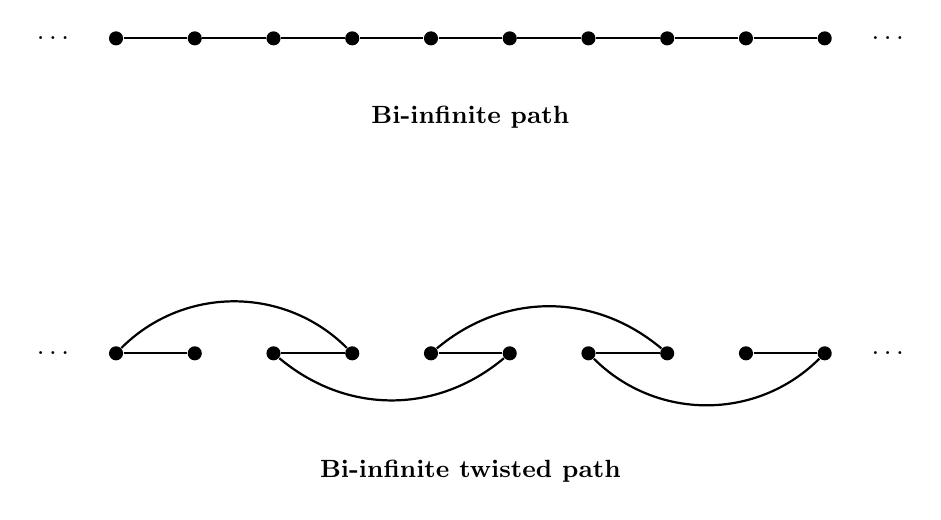
\begin{tikzpicture}[
    vertex/.style={circle, fill, inner sep=1.8pt},
    edge/.style={thick},
    caption/.style={font=\small\bfseries, node distance=1.5cm}
]

    % --- Subfigure 1: Bi-infinite Path (Top) ---
    \begin{scope}[yshift=4cm]
        % Vertices -4 to 5
        \foreach \x in {-4,...,5}
            \node[vertex] (v\x) at (\x, 0) {};
            
        % Consecutive horizontal edges
        \foreach \x [evaluate=\x as \nextx using int(\x+1)] in {-4,...,4}
            \draw[edge] (v\x) -- (v\nextx);
            
        % Continuation dots
        \node at (-4.8, 0) {$\dots$};
        \node at (5.8, 0) {$\dots$};
        
        % Caption for the first graph
        \node[caption] at (0.5, -1) {Bi-infinite path};
    \end{scope}

    % --- Subfigure 2: Matching and Arcs (Bottom) ---
    \begin{scope}[yshift=0cm]
        % Vertices -4 to 5
        \foreach \x in {-4,...,5}
            \node[vertex] (u\x) at (\x, 0) {};
            
        % Specified horizontal edges (the matching)
        \foreach \a/\b in {-4/-3, -2/-1, 0/1, 2/3, 4/5}
            \draw[edge] (u\a) -- (u\b);
            
        % Upper arcs
        \draw[edge] (u-4) to[bend left=45] (u-1);
        \draw[edge] (u0) to[bend left=40] (u3);
        
        % Lower arcs
        \draw[edge] (u-2) to[bend right=40] (u1);
        \draw[edge] (u2) to[bend right=45] (u5);

        % Continuation dots
        \node at (-4.8, 0) {$\dots$};
        \node at (5.8, 0) {$\dots$};
        
        % Caption for the second graph
        \node[caption] at (0.5, -1.5) {Bi-infinite twisted path};
    \end{scope}

\end{tikzpicture}
    \caption{Two bi-infinite paths that are isomorphic but cannot be transformed into each other using a (possibly infinite) sequence of feasible edge replacements.}
    \label{fig:infinite_paths}
\end{figure}

\begin{lemma}\label{lemma:closure_finite_witness}
    Let $\Gamma\leq S_X$ and $\varphi\in S_X$.
    Then $\varphi\in\overline{\Gamma}$ if and only if for every finite $F\subseteq X$, there is $\sigma\in\Gamma$ such that $\varphi\restriction_F=\sigma\restriction_F$.
\end{lemma}

\begin{proof}
    For the forward direction, take $\varphi$ and $F$ as above.
    Clearly, $[\varphi\restriction_F]$ is a basic open neighbourhood of $\varphi$ and hence must intersect $\Gamma$.
    Any $\sigma$ witnessing this has the sought property.

    Conversely, take an arbitrary finite partial function $t\colon F\to X$ that is extended by $\varphi$.
    Pick $\sigma\in\Gamma$ with $\varphi\restriction_F=\sigma\restriction_F$.
    Clearly, $\sigma\in\Gamma\cap[t]$, proving that $\varphi\in\overline{\Gamma}$.
\end{proof}

A group action on $X$ is called \emph{$n$-transitive} if $|X|\geq n$ and for any two pairwise distinct $n$-tuples $(x_1,\dots,x_n)$ and $(y_1,\dots,y_n)$, there is a group element $g$ such that $gx_i=y_i$ for all $1\leq i\leq n$.
Notice that $1$-transitive is just the usual definition of \emph{transitive}, i.e.\ that there is a single orbit.
If for all $n\geq1$, $\Fer(G)$ acts $n$-transitively on $X$, we say $\Fer(G)$ is \emph{highly transitive}.

\begin{proposition}\label{prop:char_local}
    The following are equivalent.
    \begin{enumerate}[label=(\arabic*)]
        \item The graph $G$ is a local amoeba.
        \item For every finite $F\subseteq X$ and every $\varphi\in S_X$, there is $\sigma\in\Fer(G)$ such that $\varphi\restriction_F=\sigma\restriction_F$.
        \item $\Fer(G)$ is highly transitive.
    \end{enumerate}
\end{proposition}

\begin{proof}
    The implication [1$\implies$2] follows from Lemma~\ref{lemma:closure_finite_witness}.
    Assume (2) and let $n\geq1$ and $(x_1,\dots,x_n)$ and $(y_1,\dots,y_n)$ be two pairwise distinct tuples.
    Let $F:=\{x_i:1\leq i\leq n\}$, then fix a bijection $X\setminus F\to X\setminus\{y_i:1\leq i\leq n\}$ (which exists since $X$ is countably infinite and these two sets differ from $X$ only in finite subsets) and define $\varphi$ such that it agrees with said bijection and in addition satisfies $\varphi(x_i)=y_i$.
    By (2), some $\sigma\in\Fer(G)$ has the desired property.

    Finally, assume (3), let $\varphi$ be an arbitrary permutation on $X$ and $F=\{x_1,\dots,x_n\}\subseteq X$.
    Apply (3) to the tuples $(x_1,\dots,x_n)$ and $(\varphi(x_1),\dots,\varphi(x_n))$ to get $\sigma\in\Fer(G)$.
    It follows that $\sigma$ agrees with $\varphi$ on $F$, hence $\varphi\in\overline{\Fer(G)}$ by Lemma~\ref{lemma:closure_finite_witness}.
    Since $\varphi$ was arbitrary, $\overline{\Fer(G)}=S_X$, that is, $G$ is a local amoeba.
\end{proof}

It is worth pointing out that in the example of the bi-infinite path, $\Fer(P_\mathbb Z)$ acts transitively on $P_\mathbb Z$ but not 2-transitively, as the same aforementioned instance shows: the pairs of labels $(0,2)$ and $(1,2)$ witness this failure.
In such cases, one could use the largest $n$ for which the group acts $n$-transitively on $V(G)$ to gauge how close $G$ is to being a local amoeba.

The next result provides an example of a graph where the gap between the automorphism group and the $\Fer$ group is as large as possible.
Concretely, the countably infinite path on $X=\omega$, denoted $P_\omega$ where the edges are given by consecutive pairs of naturals, has a trivial automorphism group, but $\Fer(P_\omega)$ is dense in $S_\omega$.

\begin{proposition}\label{prop:p_omega_local}
    $P_\omega$ is a local amoeba.
\end{proposition}

\begin{proof}
    Let $F\subseteq\omega$ be finite and $\varphi\in S_\omega$.
    Define $n:=\max(F\cup\varphi[F])+1$ and notice that $t:=\varphi\restriction_F$ is a bijection between finite subsets of $n$.
    In particular, there exists a bijection $s\colon n\setminus F\to n\setminus t[F]$.
    Now define $\sigma\colon X\to X$ by $$\sigma(x):=\begin{cases}
        s(x),&x\in n\setminus F;\\
        t(x),&x\in F;\\
        x,&x\geq n.
    \end{cases}$$ Routine arguments show that $\sigma\in S_X$.
    Now consider the induced subgraph $P_{n+1}$ and the permutation $\sigma\restriction_{n+1}$.
    Observe that this permutation fixes the endpoint of the path, $n$, by definition.
    Thus by Lemma~\ref{lemma:path-stem-symmetric}, there is a sequence $f_0,\dots,f_m$ of canonical generators of $\Fer(P_{n+1})$, all of which fix $n$, such that $\sigma\restriction_{n+1}=f_0\cdots f_m$.

    For each $i\leq m$, we can extend $f_i$ to a permutation $\overline{f_i}$ on $X$ by fixing every label $x>n$.
    Clearly, each $\overline{f_i}$ is a member of $\Fer(P_\omega)$ and thus $\sigma=\overline{f_0}\cdots\overline{f_m}\in\Fer(P_\omega)$.
    Finally, the choice of $\sigma$ makes it evident that $\sigma\restriction_F=t=\varphi\restriction_F$, and thus $P_\omega$ is a local amoeba by Proposition~\ref{prop:char_local}.
\end{proof}

In the rest of this section we restrict to trees, where the topology of the underlying graph offers extra structure (the space of ends) that controls the closed subgroups of $\Aut(T)$ and, in turn, the closure of $\Fer(T)$.

\subsection{The Freudenthal compactification of a tree and amenability}\label{subsec:freudenthal}

For the remainder of this section, $T$ denotes a countably infinite, locally finite\footnote{A graph is \emph{locally finite} if every vertex has finitely many incident edges.} tree on a label set $X$, and $\Fer(T)$ denotes the permutation group of feasible edge replacements as defined in Subsection~\ref{subsec:fer}.
The structural theory of finite trees developed in Section~\ref{sec:amoeba_trees} does not translate verbatim to this setting: Lemma~\ref{lemma:aut-fixes-vertex-or-edge}, in particular, fails for infinite trees, where there is a third type of automorphisms: \emph{translations}, which are automorphisms that fix neither vertex nor edge.
The first instance of a classification for automorphisms of locally finite trees that the author is aware of was given by Jacques Tits~\cite{Tits_1970_AutT}.

The \emph{space of ends} of a locally finite connected graph $G$ is a compactification of $G$ that captures its ``directions to infinity.''
This notion was introduced by Freudenthal~\cite{Freudenthal1942}~\cite{Freudenthal1951}.
Halin~\cite{Halin_1973_AutLocallyFiniteGraphs} studied the action of automorphisms on ends, and the topic since became a standard tool in combinatorial and geometric group theory.
We follow the presentation of Adams--Lyons~\cite{AdamsLyons_1991_AmenTreesEquiv}.

\begin{definition}[Ends]\label{def:ends}
    An \emph{end} of a tree $T$ is the equivalence class of an isometry $\pi\colon P_\omega\to T$ under the equivalence relation $\pi\sim\pi'$ if there are $n,m$ such that for all $\ell\geq0$, $\pi(m+\ell)=\pi'(n+\ell)$.
    The space of ends is called the \emph{boundary} of $T$ and denoted by $\partial T$.

    Equip $\overline T:=T\cup\partial T$ with the compact topology in which $V(T)$ is discrete and, for $S\subseteq V(T)$, the closure of $S$ in $\overline T$ is $\overline S:=S\cup\{s\in\partial T : \exists\pi\in s\ \img(\pi)\subseteq S\}$.
    Thus a neighbourhood base for $s\in\partial T$ is the collection of all $\overline S$ such that there is a finite $K\subseteq T$ with $S$ the component of $T\setminus K$ containing some representative isometry of $s$ and such that there exists $\pi\in s$ with $\img(\pi)\subseteq S$.
\end{definition}

The number of ends of a locally finite tree can take any value: a single ray $P_\omega$ has one end, the bi-infinite path $P_\mathbb Z$ has two ends, a ``comb'' tree obtained by attaching countably many disjoint rays at each vertex of a fixed ray has $\aleph_0$ ends, and the infinite $3$-regular tree has continuum-many ends.
Every automorphism of $T$ induces a homeomorphism of $\partial T$.

We briefly recall the relevant notions of amenability in the context of groups acting on trees; see~\cite{Nebbia1988} for a detailed treatment.
A locally compact group $G$ is \emph{amenable} if it admits a left-invariant mean on $L^\infty(G)$.
Compact groups and abelian groups are amenable; the free group on two generators is not.
A key criterion for non-amenability is the existence of a discrete subgroup isomorphic to the free group $F_2$.

Informally, this analytic definition is equivalent to several more combinatorial or dynamical characterizations that may be more familiar: $G$ is amenable if and only if it satisfies Følner's condition (for every compact $K\subseteq G$ and $\varepsilon>0$ there is a compact $F\subseteq G$ with $|KF\triangle F|<\varepsilon|F|$, i.e.\ $F$ is almost invariant under translation by $K$), and if and only if every continuous affine action of $G$ on a compact convex set has a fixed point.
When $G$ is discrete, a mean on $L^\infty(G)=\ell^\infty(G)$ is, via indicator functions, the same thing as a finitely additive left-invariant probability measure defined on \emph{all} subsets of $G$ -- the formulation most common in the combinatorics literature -- so the definition above specializes to that one.

For the automorphism group $\Aut(T)$ of a locally finite tree $T$, Tits~\cite{Tits_1970_AutT} proved that every automorphism $\varphi$ falls into exactly one of three types:
\begin{enumerate}
    \item \emph{Rotations:} $\varphi$ fixes a vertex $v\in V(T)$.
    \item \emph{Inversions:} $\varphi$ swaps the endpoints of an edge $\{x,y\}$.
    \item \emph{Translations:} there exists a bi-infinite line $C=\{s_n\}_{n\in\mathbb Z}$ and an integer $j\neq 0$ such that $\varphi(s_n)=s_{n+j}$ for all $n$.
\end{enumerate}
This trichotomy contrasts with the finite case (Lemma~\ref{lemma:aut-fixes-vertex-or-edge} and Corollary~\ref{cor:aut-tree-dichotomy}), where every automorphism of a finite tree is either a branch permutation (a rotation in Tits' terminology) or an edge-inversion.

Nebbia~\cite{Nebbia1988} used this classification to characterize amenability for closed subgroups of $\Aut(T)$.

\begin{theorem}[Nebbia {\cite[Theorem~1]{Nebbia1988}}]\label{thm:nebbia}
    Let $T$ be a locally finite tree and $\Gamma$ a closed subgroup of $\Aut(T)$.
    Then $\Gamma$ is amenable if and only if at least one of the following holds:
    \begin{enumerate}
        \item $\Gamma$ fixes a vertex, an edge, or a line (that is, the image of an isometry $P_\mathbb Z\to T$) set-wise in $T$;
        \item $\Gamma$ fixes an element of cardinality 1 or 2 in $\partial T$ set-wise.
    \end{enumerate}
\end{theorem}

The non-amenable case is witnessed by translations: if $\Gamma$ contains two translations $\phi$ and $\psi$ acting on two disjoint bi-infinite lines $C_1$ and $C_2$ of $T$, then $\langle\phi,\psi\rangle$ is a discrete subgroup of $\Aut(T)$ isomorphic to $F_2$.

We begin with a fact that motivates the rest of this subsection: if a feasible edge replacement on a finite tree fixes every leaf, then it must be the trivial replacement.

\begin{lemma}\label{lemma:fer-fixing-all-leaves}
    Let $T$ be a finite tree, and assume that $\sigma\in\Fer_T(e\to f)$ fixes the set of leaves $L(T)$ pointwise.
    Then $\sigma = \mathrm{id}_X$ (and thus $e=f$).
\end{lemma}

\begin{proof}
    Let $\varphi_\sigma\colon T\to T-e+f$ denote the induced isomorphism.
    The argument proceeds by induction on $|V(T)|$.

    If $|V(T)|\leq 2$, then either $T$ has no leaves (the case $|V(T)|=1$, where the conclusion is vacuous) or $T$ consists of a single edge whose two endpoints are both leaves and are fixed by hypothesis, so the conclusion is immediate.
    So suppose that $|V(T)|\geq 3$, and thus $T$ has two non-adjacent leaves; hence, $T$ has a leaf $v_\ell$ that is not an endpoint of $e$.
    Let $v_b$ denote the unique neighbour of $v_\ell$ in $T$.
    Since $\sigma(\ell)=\ell$ and $\varphi_\sigma$ preserves degrees, $v_\ell$ is also a leaf in $T-e+f$, and moreover cannot be an endpoint of $f$ either.
    Hence the unique neighbour of $v_\ell$ in $T-e+f$ is the same as in $T$, namely $v_b$, and so $\sigma(b)=b$.

    Since $v_\ell$ is not an endpoint of $e$ or $f$, removing $v_\ell$ commutes with the edge replacement, and $\varphi_\sigma$ restricts to an isomorphism $T-v_\ell\to(T-v_\ell)-e+f$.
    Hence the restriction of $\sigma$ to $X\setminus\{\ell\}$ produces a canonical generator $\sigma'\in\Fer_T(e\to f)$ of $\Fer(T-v_\ell)$.
    Every leaf of $T-v_\ell$ is either a leaf of $T$ other than $v_\ell$ or, if $\deg_T(v_b)=2$, the vertex $v_b$; in both cases, $b$ is fixed by $\sigma$.
    By induction, $\sigma$ must fix every vertex label of $T$.
\end{proof}

Unlike the finite case, when $T$ is infinite, fixing the (possibly empty) set of leaves of $T$ does not force triviality of canonical feasible edge replacements.
Indeed, the unique infinite tree where every vertex has degree $2$ except for a single vertex of degree $3$ has feasible edge replacements that are non-trivial (meaning they do move edges).

Recall that a graph is \emph{rigid} if $\overline{\Fer(G)}=A(G)$ (cf.\ Subsection~\ref{subsec:fer}).
For rigid trees, $\overline{\Fer(T)}=\overline{A(T)}=A(T)$ (the last equality holds because $A(T)$ is closed in $S_X$: each pair $i,j\in X$ contributes the clopen condition that $\sigma$ either preserves or fails to preserve the adjacency of $v_i,v_j$, and $A(T)$ is the intersection of these conditions over all pairs), and the amenability of $\overline{\Fer(T)}$ reduces to Theorem~\ref{thm:nebbia}.

\begin{proposition}\label{prop:r-regular-rigid}
    Let $T$ be the (countably infinite) $r$-regular tree, with $r\geq 2$.
    Then $\Fer(T)=A(T)$.
\end{proposition}

\begin{proof}
    Let $\sigma\in\Fer_T(e\to f)$ be a canonical generator with $e=\{u,v\}$ and $f=\{u',v'\}$.
    Since $\varphi_\sigma$ is an isomorphism $T\to T-e+f$ and $T$ is $r$-regular, $T-e+f$ is also $r$-regular.
    For each $x\in V(T)$,
    $$
        \deg_{T-e+f}(x)\;=\;r\;-\;1_{\{x\in\{u,v\}\}}\;+\;1_{\{x\in\{u',v'\}\}}.
    $$
    Equating this to $r$ for every $x$ forces $1_{\{x\in\{u,v\}\}}=1_{\{x\in\{u',v'\}\}}$, that is, $\{u,v\}=\{u',v'\}$, i.e., $e=f$.
    Hence the only canonical generators of $\Fer(T)$ are those induced by automorphisms.
\end{proof}

In particular, the infinite $r$-regular tree is rigid for every $r\geq 2$.
For $r\geq 3$, a standard fact in tree amenability is that $\Aut(T)$ contains translations on disjoint lines, whence by the discussion following Theorem~\ref{thm:nebbia}, $A(T)$ contains a copy of $F_2$ and is non-amenable.
Thus $\overline{\Fer(T)}=A(T)$ is non-amenable for these trees.

In the finite theory, a key structural result is that the canonical generators of $\Fer(T)$ arising from automorphisms of $T$ or of forests $T-e$ are accounted for by automorphisms of unicyclic graphs $T+f$.
At the group level, $\langle A(T)\cup A^-(T)\rangle\subseteq\langle A^+(T)\rangle$ (Proposition~\ref{prop:tree-A-Aminus-in-Aplus}).
The element-level inclusion $A(T)\cup A^-(T)\subseteq A^+(T)$ fails when $\Aut(T)$ contains elements of order $>2$ (see Figure~\ref{fig:counterexample_trees}), but the group-level containment still holds because every tree automorphism decomposes as a product of involutions, each of which preserves a non-edge.

For infinite trees, translations introduce a genuinely new phenomenon.
A translation $\phi_\sigma$ on a bi-infinite line $C\subseteq T$ has infinite order and moves every vertex of $C$, so no non-edge $f$ is preserved by $\phi_\sigma$.
Thus $\sigma\notin A(T+f)$ for any $f\in E(T^c)$.

That said, an infinite unicyclic graph $U=T+f$ (where $f$ is a non-edge of $T$) has a finite cycle $C$ with finitely many infinite trees hanging off the vertices of $C$.
Every automorphism of $U$ either preserves or reverses $C$ through a dihedral action, and the remaining structure is essentially a forest automorphism.
In the closure $\overline{A(U)}$, the cycle contributes at most a finite group factor: given that $C$ is finite, the restriction $\sigma\restriction_{V(C)}$ is determined by finitely many values, and the ``infinite content'' of any element of $\overline{A(U)}$ lies in its action on the branches, which are trees.
In this sense, infinite unicyclic graphs are indistinguishable from trees at infinity, and any asymptotic property of $\overline{\Fer(T)}$ that depends only on the behaviour of permutations far from a fixed finite set is unaffected by adding a single edge.

Combining the preceding observations yields a partial picture of the amenability of $\overline{\Fer(T)}$ for a countably infinite, locally finite tree $T$.
\begin{enumerate}
    \item \textbf{Local amoeba trees} (e.g., $P_\omega$): $\overline{\Fer(T)}=S_X$, which, by a standard fact, is amenable as a Polish group.
    \item \textbf{Rigid trees}: $\overline{\Fer(T)}=A(T)$, and amenability is characterized by Nebbia's Theorem~\ref{thm:nebbia}.
    The infinite $r$-regular tree, with $r\geq 3$, falls into this category by Proposition~\ref{prop:r-regular-rigid}, and its $\overline{\Fer(T)}$ is non-amenable.
    \item \textbf{Intermediate trees}: non-regular trees that are not local amoebas, such as the infinite tree with a unique vertex $v_0$ of degree $3$ and all other vertices of degree $2$.
    Here $A(T)\subsetneq\overline{\Fer(T)}\subsetneq S_X$ (to see the latter, consider $\sigma$ fixing $0$ and realizing $a\mapsto a_1$ where $a$ and $a_1$ are consecutive on some ray; the basic open set $[\sigma\restriction_{\{v_0,a\}}]$ is disjoint from $\Fer(T)$), and the amenability of $\overline{\Fer(T)}$ is not determined by either extreme case.
\end{enumerate}

\subsection{Baire-measurable colourings}\label{subsec:baire_measurable}

For uncountable $X$, the topology on $S_X$ is no longer second-countable, and in particular not sequential: a permutation $\varphi\in S_X$ may lie in the closure of a set $\Gamma\subseteq S_X$ without being a limit of any sequence in $\Gamma$.
Example~\ref{ex:aut_closure_not_seq} below exhibits this phenomenon for the automorphism group of a natural graph, foreshadowing the kind of complications one must accommodate when adapting finite combinatorial arguments to the uncountable Baire-category setting.

\begin{example}\label{ex:aut_closure_not_seq}
    Let $G$ be the graph on the vertex set $2^\omega$ with edges $\{x,y\}$ where $x\restriction_{\omega\setminus 1}\neq y\restriction_{\omega\setminus 1}$.

    Consider the map $s\colon2^\omega\to2^\omega$ that flips the first bit of an infinite binary sequence, that is, for every $x\in2^\omega$, $s(i^\frown x):=(1-i)^\frown x$.
    For each finite $s$-invariant set $F\subseteq2^\omega$, define $$\sigma_F(x):=\begin{cases}
        s(x),&x\in F;\\
        x,&x\notin F.
    \end{cases}$$

    It is straightforward to show that $\{\sigma_F:F\in[2^\omega]^{<\omega}\}\cup\{s\}\subseteq A(G)=\Fer(G)$.
    We claim that $s\in\overline{\{\sigma_F:F\in[2^\omega]^{<\omega},\,F=s[F]\}}$ but that no sequence of $\sigma_F$ converges to $s$.
    In other words, $s$ belongs to $\Fer(G)$ but is not a finite product of permutations of the form $\sigma_F$, despite being topologically close to them.

    To prove membership in the closure, let $F\subseteq 2^\omega$ be finite and consider the basic open neighbourhood $\{\varphi\in S_{2^\omega}:\varphi\restriction_F=s\restriction_F\}$ of $s$.
    The set $F':=F\cup s[F]$ is finite and $s$-invariant, and $\sigma_{F'}$ agrees with $s$ on every element of $F$ (since $F\subseteq F'$).
    Hence $\sigma_{F'}$ belongs to this neighbourhood, proving that $s\in\overline{\{\sigma_F:F\in[2^\omega]^{<\omega},\,F=s[F]\}}$.

    Now, consider any sequence $\{F_n:n<\omega\}$ of finite subsets of the Cantor space.
    Since each $F_n$ is finite, the union $\bigcup_n F_n$ is countable; as $2^\omega$ is uncountable, there exists a binary sequence $x$ that is not in any $F_n$.
    Therefore, the pointwise limit $\lim_{n\to\infty}\sigma_{F_n}(x)=x$ differs from $s(x)$ at the first bit and thus cannot be equal.
\end{example}

In the finite setting, a $2$-edge-colouring of $K_n$ contains a balanced copy of a balanceable graph $G$ provided each colour class has more than $\bal(n,G)$ edges.
The natural Baire-category transposition of ``many edges of each colour'' is ``non-meagre colour classes,'' and the goal of this subsection is to show that two of the central finite results of the previous sections, namely Theorem~\ref{thm:constant_bal} and Theorem~\ref{thm:bal_eq_ex}, have infinitary analogues.
 
The proofs share the following localization lemma.
A subtlety, absent in the finite theory, is that the localization is necessarily \emph{off-diagonal}: it produces a pair of disjoint open sets whose cross-pair set carries a comeagre colour class, rather than a single open set on whose full pair-set the colour is comeagre.
This phenomenon is unavoidable.
For example, let $X=(0,1)$ and define a colouring $$c\colon[X]^2\to 2\quad\text{ by }\quad c(x,y)=0\iff|\{x,y\}\cap (0,1/2)|=1.$$
Then both colour classes are open and non-meagre.
However, for every non-empty open set $U\subseteq X$, either:
\begin{itemize}
    \item $U\subseteq (0,1/2)$ or $U\subseteq (1/2,1)$, in which case $[U]^2$ is monochromatic; or
    \item $U$ meets both halves of $(0,1)$, in which case both colours occur on non-meagre open subsets of $[U]^2$.
\end{itemize}
Thus no colour class is comeagre on every $[U]^2$.
 
\begin{lemma}\label{lemma:graph_localization}
    Let $X$ be a perfect Polish space, and let $\pi\colon X^2\setminus\Delta\to [X]^2$ denote the quotient map.
    Given disjoint non-meagre sets $A,B\subseteq [X]^2$ with the Baire property, there exist pairwise disjoint non-empty open sets $U_A^1,U_A^2,U_B^1,U_B^2\subseteq X$ such that $A$ is comeagre in $\pi[U_A^1\times U_A^2]$ and $B$ is comeagre in $\pi[U_B^1\times U_B^2]$.
\end{lemma}
 
\begin{proof}
    Since $A$ and $B$ have the Baire property, there exist open sets $O_A,O_B\subseteq [X]^2$ such that $A\Delta O_A$ and $B\Delta O_B$ are meagre.
    Because $A$ and $B$ are non-meagre, the sets $O_A$ and $O_B$ are non-empty.
    Moreover, $O_A\cap O_B\subseteq(A\Delta O_A)\cup(B\Delta O_B)$, since $A\cap B=\emptyset$.
    Hence $O_A\cap O_B$ is meagre as well.
    But $O_A\cap O_B$ is open in the Polish space $[X]^2$, so by the Baire category theorem, $O_A\cap O_B=\emptyset$.
 
    Let $$\mathcal O_A:=\pi^{-1}[O_A],\qquad\mathcal O_B:=\pi^{-1}[O_B].$$
    These are disjoint non-empty open subsets of $X^2\setminus\Delta$.
    Choose $(\alpha_1,\alpha_2)\in \mathcal O_A$.
    Since $\alpha_1\neq \alpha_2$ and $X$ is metrizable, there exist disjoint open neighbourhoods $$V_A^1\ni \alpha_1,\qquad V_A^2\ni \alpha_2$$ such that $V_A^1\times V_A^2\subseteq \mathcal O_A$.
    Similarly, choose disjoint non-empty open sets $V_B^1,V_B^2\subseteq X$ with $V_B^1\times V_B^2\subseteq \mathcal O_B$.
    Since $X$ is perfect, every non-empty open set is infinite.
    Pick points $a_1\in V_A^1$ and $a_2\in V_A^2$.
    Since $V_A^1\cap V_A^2=\emptyset$, we have $a_1\neq a_2$; then $b_1\in V_B^1\setminus\{a_1,a_2\}$, possible by perfectness; finally $b_2\in V_B^2\setminus\{a_1,a_2,b_1\}$, again by perfectness.
    The four points $a_1,a_2,b_1,b_2\in X$ are pairwise distinct by construction.
    Using metrizability again, choose pairwise disjoint open neighbourhoods $$U_A^1\ni a_1,\quad U_A^2\ni a_2,\quad U_B^1\ni b_1,\quad U_B^2\ni b_2$$ such that $$U_A^1\subseteq V_A^1,\quad U_A^2\subseteq V_A^2,\quad U_B^1\subseteq V_B^1,\quad U_B^2\subseteq V_B^2.$$
    Then $$\pi[U_A^1\times U_A^2]\subseteq O_A,\qquad\pi[U_B^1\times U_B^2]\subseteq O_B.$$
    
    Now $$\pi[U_A^1\times U_A^2]\setminus A\subseteq O_A\setminus A\subseteq A\Delta O_A,$$ and $A\Delta O_A$ is meagre in $[X]^2$.
    Since $U_A^1$ and $U_A^2$ are disjoint, $U_A^1\times U_A^2\subseteq X^2\setminus\Delta$, and therefore $\pi[U_A^1\times U_A^2]$ is open in $[X]^2$.
    Since $\pi[U_A^1\times U_A^2]$ is open in $[X]^2$, the subset $\pi[U_A^1\times U_A^2]\setminus A$ is meagre in $\pi[U_A^1\times U_A^2]$ as well.
    Hence $A$ is comeagre in $\pi[U_A^1\times U_A^2]$.
    The same argument applies to $B$.
\end{proof}
 
We recall the following classical theorem of Galvin.
 
\begin{fact}[Galvin]\label{fact:galvin}
    Let $X$ be a perfect Polish space and let $c\colon[X]^2\to k$ be a Baire-measurable colouring with finitely many colours.
    Then there exists a Cantor set $C\subseteq X$ such that $[C]^2$ is monochromatic.
\end{fact}
 
A proof may be found in~\cite[Theorem~19.6]{Kechris_1995_DescriptiveSetTheory}.
We shall also use the following product form of Mycielski's theorem.
 
\begin{fact}[Product Mycielski]\label{fact:product_mycielski}
    Let $X,Y$ be perfect Polish spaces, let $U\subseteq X$ and $V\subseteq Y$ be non-empty open sets, and let $R\subseteq U\times V$ have the Baire property and be comeagre in $U\times V$.
    Then there exist Cantor sets $C\subseteq U,\qquad D\subseteq V$ such that $C\times D\subseteq R$.
\end{fact}
 
\begin{proof}[Proof sketch]
    Write $(U\times V)\setminus R=\bigcup_n M_n$ with each $M_n$ nowhere dense.
    A standard fusion construction simultaneously builds binary trees of open sets $$\{U_s:s\in 2^{<\omega}\}\subseteq U,\qquad\{V_s:s\in 2^{<\omega}\}\subseteq V,$$ with shrinking diameters and pairwise disjoint successors, while ensuring that for every $k$ and every $s,t\in 2^k$, $\overline{U_s}\times\overline{V_t}\cap M_k=\emptyset$.
    The resulting limit sets $C,D$ are Cantor sets satisfying $C\times D\subseteq R$.
\end{proof}
 
The next lemma is the key extraction step.
 
\begin{lemma}[Joint Cantor extraction]\label{lemma:joint_extraction}
    Let $X$ be a perfect Polish space, let $U^1,U^2\subseteq X$ be disjoint non-empty open sets, and let $c\colon[X]^2\to 2$ be a Baire-measurable colouring such that $c^{-1}\{\mathrm{red}\}$ is comeagre in $\pi[U^1\times U^2]$.
    Then there exist Cantor sets $$D^1\subseteq U^1,\qquad D^2\subseteq U^2$$ such that:
    \begin{enumerate}[label=\textup{(\roman*)}]
        \item $[D^1]^2$ is monochromatic;
        \item $[D^2]^2$ is monochromatic;
        \item $c(x,y)=\mathrm{red}$ for all $x\in D^1$ and $y\in D^2$.
    \end{enumerate}
\end{lemma}
 
\begin{proof}
    Define $R:=\{(x,y)\in U^1\times U^2:c(x,y)=\mathrm{red}\}$.
    Since $c^{-1}\{\mathrm{red}\}$ is comeagre in $\pi[U^1\times U^2]$, and $\pi\colon U^1\times U^2\to \pi[U^1\times U^2]$ is continuous and open, the set $R$ is comeagre in $U^1\times U^2$.
    Moreover, $R$ has the Baire property because $c$ is Baire measurable.
    
    Applying Fact~\ref{fact:product_mycielski}, there exist Cantor sets $$P^1\subseteq U^1,\qquad P^2\subseteq U^2$$ such that $P^1\times P^2\subseteq R$.
    Equivalently, $c(x,y)=\mathrm{red}\quad\text{for all } x\in P^1,\ y\in P^2$.
    
    Now apply Fact~\ref{fact:galvin} to the restriction $c\restriction_{[P^1]^2}$.
    There exists a Cantor set $D^1\subseteq P^1$ such that $[D^1]^2$ is monochromatic.
    
    Similarly, applying Fact~\ref{fact:galvin} to $c\restriction_{[P^2]^2}$, there exists a Cantor set $$D^2\subseteq P^2$$ such that $[D^2]^2$ is monochromatic.
    Since $D^1\times D^2\subseteq P^1\times P^2\subseteq R$, every cross-pair between $D^1$ and $D^2$ is red.
\end{proof}
 
\begin{remark}\label{rmk:joint_extraction_symmetric}
    The statement of Lemma~\ref{lemma:joint_extraction} is symmetric in the two colours: its hypothesis and conclusion exchange under the swap $\mathrm{red}\leftrightarrow\mathrm{blue}$.
    Hence the lemma may equally be applied with blue in the role of the comeagre colour, the conclusion then being that every cross-pair is blue.
\end{remark}
 
We will also use a trivial discrete intermediate value theorem.
 
\begin{lemma}[Discrete IVT]\label{lemma:discrete_ivt}
    Let $(\ell_i)_{i=0}^t$ be a sequence of integers with $\ell_0=a$, $\ell_t=b$, and $|\ell_{i+1}-\ell_i|\leq 1$ for all $i$.
    Then every integer between $a$ and $b$ inclusive is equal to some $\ell_i$.
\end{lemma}
 
\paragraph{An infinitary analogue of constant balancing.}
 
Theorem~\ref{thm:constant_bal} characterizes graphs of constant balancing number as those admitting both a matching $\frac{k}{2}K_2$ and a star $K_{1,k/2}$.
The result below is the natural Baire-category analogue: every non-meagre Baire-measurable $2$-colouring of $[X]^2$ on a perfect Polish space contains both a monochromatic Cantor clique in one colour and a Cantor-indexed star in the other colour.
 
\begin{theorem}\label{thm:inf_const_bal}
    Let $X$ be a perfect Polish space and suppose that $c\colon[X]^2\to 2$ is a Baire-measurable colouring whose colour classes are non-meagre.
    Then there exist a colour $i<2$, a vertex $v_0\in X$, and a Cantor set $C\subseteq X$ such that:
    \begin{enumerate}[label=\textup{(\roman*)}]
        \item $c(v_0,x)=i$ for every $x\in C$;
        \item $[C]^2$ is monochromatic in colour $1-i$.
    \end{enumerate}
    In particular, $[C]^2$ contains a matching of cardinality continuum in colour $1-i$.
\end{theorem}
 
\begin{proof}
    Apply Lemma~\ref{lemma:graph_localization} with $$A:=c^{-1}\{\mathrm{red}\},\qquad B:=c^{-1}\{\mathrm{blue}\},$$ to obtain pairwise disjoint non-empty open sets $U_A^1,U_A^2,U_B^1,U_B^2\subseteq X$ such that red is comeagre in $\pi[U_A^1\times U_A^2]$ and blue is comeagre in $\pi[U_B^1\times U_B^2]$.
    Apply Lemma~\ref{lemma:joint_extraction} on the $A$-side.
    We obtain Cantor sets $$D_A^1\subseteq U_A^1,\qquad D_A^2\subseteq U_A^2$$ such that:
    \begin{itemize}
        \item every cross-pair between $D_A^1$ and $D_A^2$ is red;
        \item each of $[D_A^1]^2$ and $[D_A^2]^2$ is monochromatic.
    \end{itemize}
 
    Let $j_A^1,j_A^2\in\{\mathrm{red},\mathrm{blue}\}$ denote the colours of $[D_A^1]^2$ and $[D_A^2]^2$ respectively.
 
    \medskip\noindent\textit{Case 1.}\quad At least one of $j_A^1,j_A^2$ equals $\mathrm{blue}$.
    
    Concretely:
    \begin{itemize}
        \item if $j_A^2=\mathrm{blue}$, fix $v_0\in D_A^1$ and let $C:=D_A^2$;
        \item if $j_A^1=\mathrm{blue}$ and $j_A^2=\mathrm{red}$, fix $v_0\in D_A^2$ and let $C:=D_A^1$;
        \item if $j_A^1=j_A^2=\mathrm{blue}$, either choice works; pick $v_0\in D_A^1$ and $C:=D_A^2$.
    \end{itemize}
    In each configuration, every edge between $v_0$ and a point of $C$ is a cross-pair between $D_A^1$ and $D_A^2$, hence red, while $[C]^2$ is monochromatic blue.
    Set $i:=\mathrm{red}$.
 
    \medskip\noindent\textit{Case 2.}\quad $j_A^1=j_A^2=\mathrm{red}$.
    
    By Remark~\ref{rmk:joint_extraction_symmetric}, we may apply Lemma~\ref{lemma:joint_extraction} on the $B$-side with blue in the role of the comeagre colour.
    We obtain Cantor sets $$D_B^1\subseteq U_B^1,\qquad D_B^2\subseteq U_B^2$$ such that:
    \begin{itemize}
        \item every cross-pair between $D_B^1$ and $D_B^2$ is blue;
        \item each of $[D_B^1]^2$ and $[D_B^2]^2$ is monochromatic.
    \end{itemize}
    Let $j_B^1,j_B^2$ denote the corresponding clique colours.
    
    \medskip\noindent\textit{Subcase 2.1.}\quad At least one of $j_B^1,j_B^2$ equals $\mathrm{red}$.
    
    By the analogue of Case~1 with the roles of red and blue swapped:
    \begin{itemize}
        \item if $j_B^2=\mathrm{red}$, fix $v_0\in D_B^1$ and let $C:=D_B^2$;
        \item if $j_B^1=\mathrm{red}$ and $j_B^2=\mathrm{blue}$, fix $v_0\in D_B^2$ and let $C:=D_B^1$;
        \item if $j_B^1=j_B^2=\mathrm{red}$, pick $v_0\in D_B^1$ and $C:=D_B^2$.
    \end{itemize}
    In each configuration, every edge between $v_0$ and a point of $C$ is a cross-pair between $D_B^1$ and $D_B^2$, hence blue, while $[C]^2$ is monochromatic red.
    Set $i:=\mathrm{blue}$.
 
    \medskip\noindent\textit{Subcase 2.2.}\quad $j_B^1=j_B^2=\mathrm{blue}$.
    
    In this configuration $D_A^1\cup D_A^2$ is an all-red Cantor clique and $D_B^1\cup D_B^2$ is an all-blue Cantor clique, but the cross-colour between the two sides has not yet been controlled.
    We extract a controlled cross between $D_A^1$ and $D_B^1$ via the Baire property and Fact~\ref{fact:product_mycielski}.
 
    Since $c$ is Baire-measurable, the two colour classes partition $\pi[D_A^1\times D_B^1]$ into sets with the Baire property, at least one of which is non-meagre in $D_A^1\times D_B^1$.
    Let $k\in\{\mathrm{red},\mathrm{blue}\}$ denote the non-meagre colour.
    Since $D_A^1$ and $D_B^1$ are Cantor sets, they are themselves perfect Polish spaces in the subspace topology.
    Thus there exist relatively open non-empty sets $W_A\subseteq D_A^1$ and $W_B\subseteq D_B^1$ such that $c^{-1}\{k\}$ is comeagre in $W_A\times W_B$.
    Applying Fact~\ref{fact:product_mycielski} inside the perfect Polish spaces $D_A^1$ and $D_B^1$, we obtain Cantor sets $$\widetilde D_A\subseteq W_A\subseteq D_A^1,\qquad\widetilde D_B\subseteq W_B\subseteq D_B^1$$ such that $\widetilde D_A\times\widetilde D_B\subseteq c^{-1}\{k\}$.
    Hence every cross-pair between $\widetilde D_A$ and $\widetilde D_B$ has colour $k$.
 
    If $k=\mathrm{red}$, fix any $v_0\in\widetilde D_A$ and let $C:=\widetilde D_B$.
    Then every edge between $v_0$ and $C$ is red, while $[C]^2\subseteq [D_B^1]^2$ is monochromatic blue.
    Set $i:=\mathrm{red}$.
 
    If $k=\mathrm{blue}$, fix any $v_0\in\widetilde D_B$ and let $C:=\widetilde D_A$.
    Then every edge between $v_0$ and $C$ is blue, while $[C]^2\subseteq [D_A^1]^2$ is monochromatic red.
    Set $i:=\mathrm{blue}$.
 
    \medskip
    
    The cases above exhaust all possibilities for $(j_A^1,j_A^2)$ and $(j_B^1,j_B^2)$, and in every case the resulting $v_0,C,i$ satisfy conditions (i) and (ii).
    Finally, if $C$ is any Cantor set such that $[C]^2$ is monochromatic in colour $1-i$, then $[C]^2$ contains a matching of cardinality continuum in colour $1-i$: fixing a homeomorphism $\varphi\colon 2^\omega\to C$, the family $$\bigl\{\{\varphi(0^\frown x),\varphi(1^\frown x)\}:x\in 2^\omega\bigr\}$$ is a pairwise vertex-disjoint family of monochromatic edges of cardinality $2^{\aleph_0}$.
\end{proof}
 
\paragraph{An infinitary analogue of $\bal(n,G)=\ex(n,\mathcal H_G)$.}
 
Theorem~\ref{thm:bal_eq_ex} expresses the balancing number of a global amoeba as a Tur\'an-type threshold.
Its upper-bound direction asserts that sufficiently dense red and blue edge sets force a balanced copy of the target graph.
The theorem below is the corresponding Baire-category statement: replacing positive density by non-meagreness of the colour classes forces a balanced copy of every finite global amoeba.
 
\begin{theorem}\label{thm:inf_bal_eq_ex}
    Let $X$ be a perfect Polish space, let $G$ be a finite global amoeba on $n\geq 1$ vertices and $m$ edges, and let $c\colon[X]^2\to 2$ be a Baire-measurable colouring with non-meagre colour classes.
    Then $K_X$, with the colouring $c$, contains a balanced copy of $G$.
\end{theorem}
 
\begin{proof}
    The result is trivial when $m\leq 1$, so assume that $m\geq 2$.
 
    By the global amoeba property of $G$, there exists an integer $N\geq n$ such that any two copies of $G$ in $K_{2N}$ are connected by a chain of feasible edge replacements.
 
    Apply Lemma~\ref{lemma:graph_localization} to the colour classes to obtain pairwise disjoint non-empty open sets $$U_A^1,U_A^2,U_B^1,U_B^2$$ such that red is comeagre in $\pi[U_A^1\times U_A^2]$ and blue is comeagre in $\pi[U_B^1\times U_B^2]$.
    
    Apply Lemma~\ref{lemma:joint_extraction} on the $A$-side.
    We obtain Cantor sets $$D_A^1\subseteq U_A^1,\qquad D_A^2\subseteq U_A^2$$ such that:
    \begin{itemize}
        \item every cross-pair between $D_A^1$ and $D_A^2$ is red;
        \item each of $[D_A^1]^2$ and $[D_A^2]^2$ is monochromatic.
    \end{itemize}
 
    Let $j_A^1,j_A^2\in\{\mathrm{red},\mathrm{blue}\}$ denote the colours of $[D_A^1]^2$ and $[D_A^2]^2$ respectively.
 
    \medskip
 
    \noindent\textit{Case 1.}
    $\{j_A^1,j_A^2\}=\{\mathrm{red},\mathrm{blue}\}$.
    Without loss of generality, $$j_A^1=\mathrm{red},\qquad j_A^2=\mathrm{blue}.$$
    Choose sets $V_R\subseteq D_A^1$ and $V_B\subseteq D_A^2$ each of cardinality $N$, and set $$V:=V_R\cup V_B.$$
    Then:
    \begin{itemize}
        \item every edge inside $V_R$ is red;
        \item every edge inside $V_B$ is blue;
        \item every cross-edge between $V_R$ and $V_B$ is red.
    \end{itemize}
 
    Choose copies $G_R,G_B\subseteq K_V$ of $G$ with $$V(G_R)\subseteq V_R,\qquad V(G_B)\subseteq V_B.$$
    Then all edges of $G_R$ are red and all edges of $G_B$ are blue.
    By the choice of $N$, there exists a chain $G_R=H_0,H_1,\dots,H_t=G_B$ of copies of $G$ in $K_V$ such that each $H_{i+1}$ is obtained from $H_i$ by a feasible edge replacement.
 
    Let $\ell_i$ denote the number of red edges of $H_i$.
    Then $\ell_0=m$, $\ell_t=0$, and $|\ell_{i+1}-\ell_i|\leq 1$ for every $i$.
    By Lemma~\ref{lemma:discrete_ivt}, some $H_i$ satisfies $\ell_i\in\{\lfloor m/2\rfloor,\lceil m/2\rceil\}$, hence is balanced.
 
    \medskip
 
    \noindent\textit{Case 2.}
    $j_A^1=j_A^2=\mathrm{blue}$.
 
    Choose sets $V_1\subseteq D_A^1$ and $V_2\subseteq D_A^2$ each of cardinality $N$, and set $V:=V_1\cup V_2$.
    Then:
    \begin{itemize}
        \item every edge inside $V_1$ or $V_2$ is blue;
        \item every cross-edge between $V_1$ and $V_2$ is red.
    \end{itemize}
 
    Let $G^{(1)}$ be a copy of $G$ inside $V_1$.
    Then every edge of $G^{(1)}$ is blue, so the number of red edges equals $0$.
    Next choose a partition $V(G)=L\sqcup R$ realizing $\mathrm{MaxCut}(G)$.
    By the classical probabilistic argument of Erd\H{o}s, $\mathrm{MaxCut}(G)\geq \frac{m}{2}$, hence $\mathrm{MaxCut}(G)\geq \lceil m/2\rceil$.
    Choose an injection $\iota\colon V(G)\to V$ with $\iota[L]\subseteq V_1$ and $\iota[R]\subseteq V_2$.
    Let $G^{(2)}$ denote the image copy of $G$ under $\iota$.
    Then, $G^{(2)}$ has exactly $\mathrm{MaxCut}(G)$ red edges.
 
    Now connect $G^{(1)}$ and $G^{(2)}$ by a sequence of feasible edge replacements inside $K_V$.
    The number of red edges begins at $0$ and ends at at least $\lceil m/2\rceil$, changing by at most $1$ at each step.
    Lemma~\ref{lemma:discrete_ivt} therefore yields a balanced copy of $G$.
 
    \medskip
 
    \noindent\textit{Case 3.}
    $j_A^1=j_A^2=\mathrm{red}$.
    Applying Lemma~\ref{lemma:joint_extraction} on the $B$-side (with blue in the role of the comeagre colour, by Remark~\ref{rmk:joint_extraction_symmetric}), we obtain Cantor sets $D_B^1\subseteq U_B^1$ and $D_B^2\subseteq U_B^2$ such that:
    \begin{itemize}
        \item every cross-pair between $D_B^1$ and $D_B^2$ is blue;
        \item each of $[D_B^1]^2$ and $[D_B^2]^2$ is monochromatic.
    \end{itemize}
 
    Let $j_B^1,j_B^2$ denote the corresponding clique colours.
 
    \medskip
 
    \noindent\textit{Subcase 3.1.}
    $\{j_B^1,j_B^2\}=\{\mathrm{red},\mathrm{blue}\}$.
    This is symmetric to Case~1 with the roles of red and blue reversed.
 
    \medskip
 
    \noindent\textit{Subcase 3.2.}
    $j_B^1=j_B^2=\mathrm{red}$.
    This is symmetric to Case~2 with the roles of red and blue reversed.
 
    \medskip
 
    \noindent\textit{Subcase 3.3.}
    $j_B^1=j_B^2=\mathrm{blue}$.
    Choose sets $V_R\subseteq D_A^1$ and $V_B\subseteq D_B^1$ each of cardinality $N$.
    Then every edge inside $V_R$ is red and every edge inside $V_B$ is blue.
    Choose copies $G_R\subseteq K_{V_R}$ and $G_B\subseteq K_{V_B}$ of $G$.
    Then all edges of $G_R$ are red and all edges of $G_B$ are blue.
    By the choice of $N$, there exists a sequence of feasible edge replacements $G_R=H_0,\dots,H_t=G_B$ inside $K_{V_R\cup V_B}$.
    The number of red edges decreases from $m$ to $0$ in steps of size at most $1$, so Lemma~\ref{lemma:discrete_ivt} yields a balanced copy.
    The cases above exhaust all possibilities, completing the proof.
\end{proof}
 
\begin{remark}
    Theorem~\ref{thm:inf_const_bal} and Theorem~\ref{thm:inf_bal_eq_ex} are different in character.
    The former produces explicit infinitary structure: a Cantor-indexed monochromatic star together with a monochromatic Cantor clique in the opposite colour in every non-meagre Baire-measurable colouring.
    The latter instead uses the finite global amoeba structure of the target graph $G$ to interpolate between monochromatic copies via feasible edge replacements.
 
    Both arguments rely on the localization lemma together with Galvin's theorem and product forms of Mycielski's theorem.
\end{remark}
